\section{\textbf{Evaluation}}\label{sec:5}

	First of all the breadboard circuit~\ref{fig:proto_board} was tested using a multimeter to ensure it's proper functionality. With Q1 and Q2 activated the voltage measured across the motor was $3.8\;V$ \todo{review values}, for future analysis this situation (Q1 and Q2 active) will be called S1. With Q3 and Q4 activated the voltage measured was $-2.9\;V$, this will be the S2 situation. The polarity inversion was accomplished, however the magnitude for both cases which was expected to be equal was in fact different. A slightly tension drop occurred when the current flew backwards \todo{explain why. idk why}. \todo{ADDITIONAL: MEASURE MOTOR SPIN SPEED}
	
	Despite the previous mentioned discrepancy the circuit performed as intentioned therefore the motor was plugged into the circuit. For S1 the motor spun in the counterclockwise direction. On the other hand for S2 it spun clockwise slightly slower, as a result of the voltage drop previous mentioned.
	
	Finally with the printed circuit board in hands the tension across the output pins were once again measured with a voltmeter. In case S1 the voltage showed up to be \todo{MEASURE THIS!!!}. Though for S2 the tension measured was \todo{measure}. As the PCB performed exactly as the breadboard circuit the motor was connected and the final configuration was achieved. \todo{measure motor speed and direction and insert here}

\begin{figure}[t]
\centering
\centering%
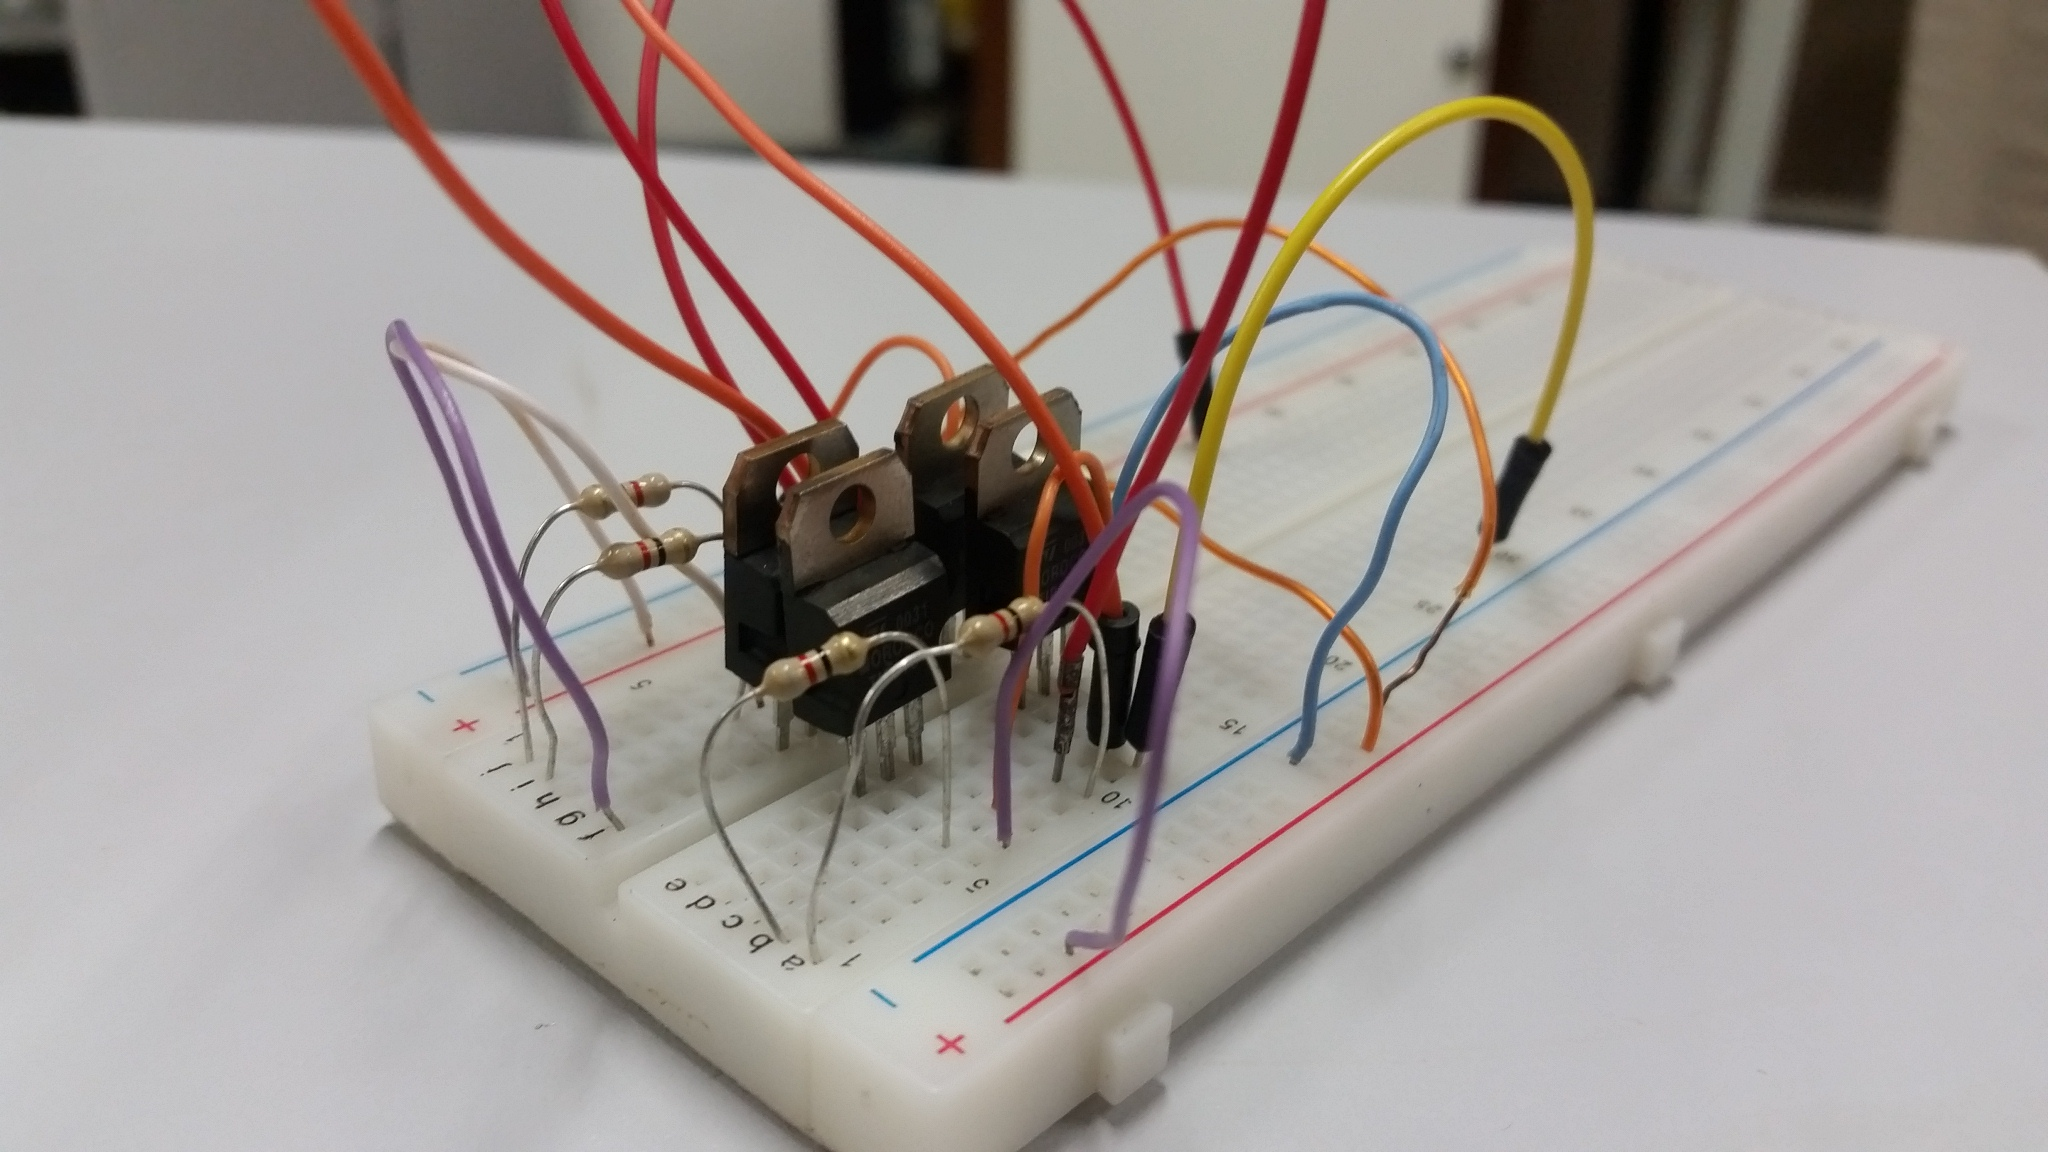
\includegraphics[height=.30\textwidth]{img/h_bridge_proto_close.jpg}
\caption{H bridge on breadboard.}
\label{fig:proto_board}%
\end{figure}
